\begin{example}~
\label{ex:single_modulated}
	Assume the set of confidential information is given as $P = \set{(1,3),(2,1),(3,4),(4,1),(5,5),(6,9)}$. In order to obscure the transmission of the information, \AgentOne modulates the confidential information by a relation represented by $M = \set{(0,9),(1,0),(2,1),(3,2),(4,3),(5,4),(6,5),(7,6),(8,7),(9,8)}$ prior to its encryption. Then, the new relation representing the confidential information is given by $(\RAcompose{P}{M}) = \set{(1,2),(2,0),(3,3),(4,0),(5,4),(6,8)}$. This information is encrypted and sent on a single communication channel as $Q = \set{(1,11),(2,0),(3,12),(4,0),(5,16),\\(6,8)}$.  \newline 

	We define the relations $P$, $M$ and $Q$ in \relview\ as follows: \newline

	\begin{figure}[ht]
		\centering
		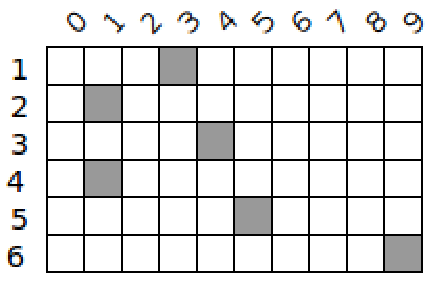
\includegraphics[scale=0.65]{Figures/PDF/Relview/P.pdf}
		\caption{Relation $P$ for Example~\ref{ex:single_modulated}.}
		\label{fig:single_modulated_p}
	\end{figure}
	
	\begin{figure}[ht]
		\centering
		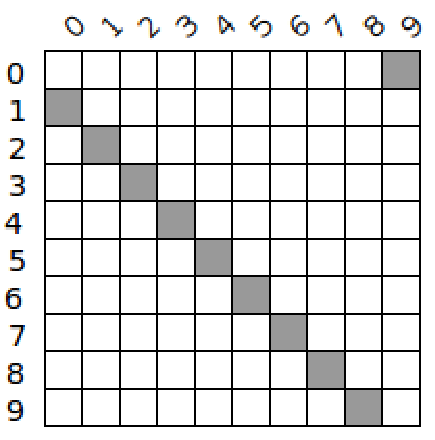
\includegraphics[scale=0.65]{Figures/PDF/Relview/NoiseP.pdf}
		\caption{Modulation relation $M$ for Example~\ref{ex:single_modulated}.}
		\label{fig:single_modulated_s}
	\end{figure}
	
	\begin{figure}[ht]
		\centering
		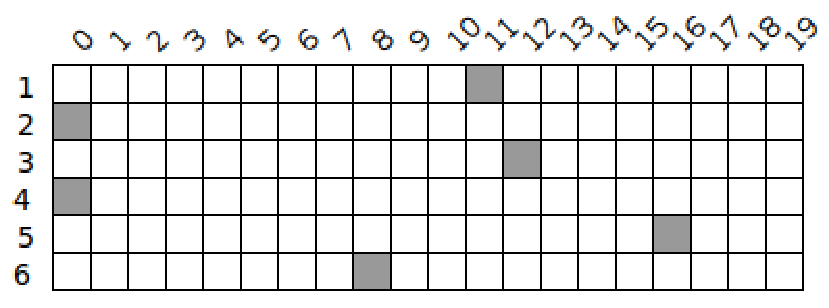
\includegraphics[scale=0.65]{Figures/PDF/Relview/Qmod.pdf}
		\caption{Relation $Q$ for Example~\ref{ex:single_modulated}.}
		\label{fig:single_modulated_q}
	\end{figure}
	\newpage

	The modulated confidential information is represented in \relview\ as follows: \newline
	
	\begin{figure}[ht]
		\centering
		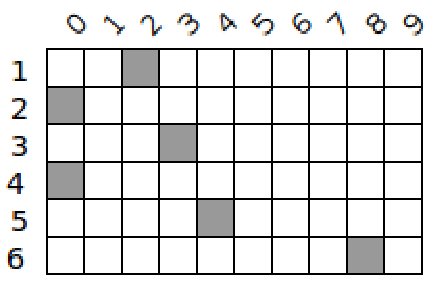
\includegraphics[scale=0.65]{Figures/PDF/Relview/PNoiseP.pdf}
		\caption{Relation $(\RAcompose{P}{M})$ for Example~\ref{ex:single_modulated}.}
		\label{fig:single_modulated_ps}
	\end{figure}
	
	We verify the existence of an abstraction relation by executing Program~\ref{prog:test} ($Result = Test(P, Q)$). In this case we are looking for an abstraction relation relating the confidential information, $P$, and the information sent on the communication channel, $Q$, which corresponds to the encrypted modulated confidential information. \newline

	\begin{figure}[ht]
		\centering
		
\includegraphics[scale=0.65]{Figures/PDF/Relview/True.pdf}
		\caption{Relation $Result$ for Example~\ref{ex:single_modulated}.}
		\label{fig:single_modulated_result}
	\end{figure}

	Therefore, the test has passed so we can compute the abstraction relation by executing Program~\ref{prog:compute} ($X = Compute(P,Q,R)$) where $R$ is the filtering relation. \newline

	\begin{figure}[ht]
		\centering
		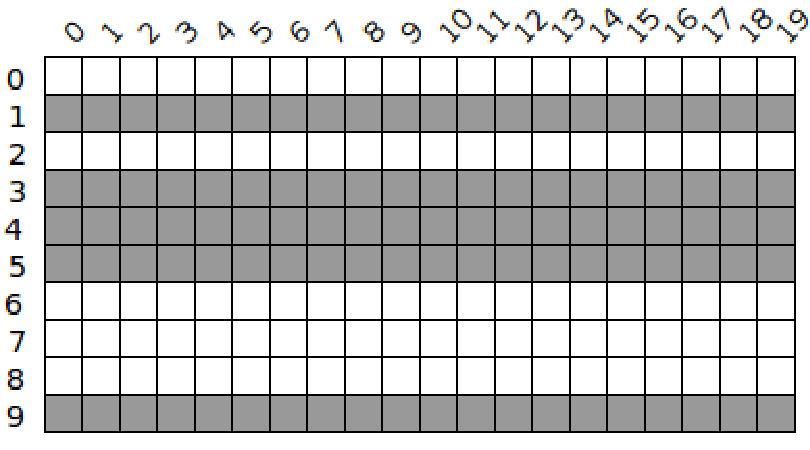
\includegraphics[scale=0.65]{Figures/PDF/Relview/R.pdf}
		\caption{Filtering relation $R$ for Example~\ref{ex:single_modulated}.}
		\label{fig:single_modulated_r}
	\end{figure}
	
	\begin{figure}[ht]
		\centering
		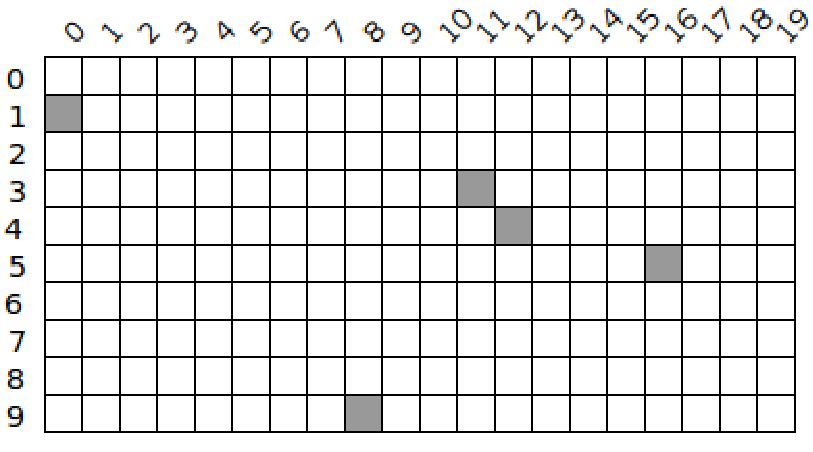
\includegraphics[scale=0.65]{Figures/PDF/Relview/XNP.pdf}
		\caption{Abstraction relation $X$ for Example~\ref{ex:single_modulated}.}
		\label{fig:single_modulated_x}
	\end{figure}
	
	\newpage
\end{example}